\documentclass[12pt]{article}
\usepackage[a4paper,margin=2.5cm]{geometry}
\usepackage{mathptmx}
\usepackage{setspace}
\onehalfspacing
\usepackage{graphicx}
\usepackage{longtable}
\usepackage{array}
\usepackage{booktabs}
\usepackage{hyperref}
\usepackage{xcolor}
\usepackage{listings}
\usepackage{tikz}
\usetikzlibrary{positioning,arrows.meta,shapes.geometric,fit,backgrounds,calc,decorations.pathreplacing}
\usepackage{float}
\usepackage{enumitem}
\usepackage{fancyhdr}
\usepackage{titlesec}
\usepackage[title]{appendix}

\hypersetup{
  colorlinks=true,
  linkcolor=blue!70!black,
  urlcolor=blue!60!black,
  citecolor=green!50!black
}

\lstset{
  basicstyle=\ttfamily\small,
  breaklines=true,
  frame=single,
  backgroundcolor=\color{gray!8},
  keywordstyle=\color{blue!70!black},
  commentstyle=\color{green!50!black},
  stringstyle=\color{red!60!black},
  numbers=left,
  numberstyle=\tiny\color{gray},
  numbersep=5pt,
  showstringspaces=false,
  tabsize=2
}

\pagestyle{fancy}
\fancyhf{}
\fancyhead[L]{\small\leftmark}
\fancyhead[R]{\small MHM Pipeline --- Project Definition}
\fancyfoot[C]{\thepage}
\renewcommand{\headrulewidth}{0.4pt}

\titleformat{\section}{\Large\bfseries}{\thesection}{1em}{}
\titleformat{\subsection}{\large\bfseries}{\thesubsection}{1em}{}
\titleformat{\subsubsection}{\normalsize\bfseries}{\thesubsubsection}{1em}{}

\newcommand{\filepath}[1]{\texttt{\small #1}}
\newcommand{\code}[1]{\texttt{#1}}

\title{%
  \vspace{-1cm}
  {\LARGE\bfseries Mapping Hebrew Manuscripts (MHM)}\\[0.5cm]
  {\LARGE\bfseries MARC-to-RDF Conversion Pipeline}\\[0.5cm]
  {\Large Project Definition Document}\\[1cm]
  {\large Version 1.1}
}
\author{
  Alexander Goldberg\\
  Department of Information Science and Applied Artificial Intelligence\\
  Bar-Ilan University, Ramat-Gan 5290002, Israel\\[4pt]
  \href{mailto:alexander.goldberg@biu.ac.il}{alexander.goldberg@biu.ac.il}\\
  \href{https://orcid.org/0009-0004-5967-9377}{ORCID: 0009-0004-5967-9377}\\[0.5cm]
  Supervisor: Prof.\ Gila Prebor\\
  \href{mailto:gila.prebor@biu.ac.il}{gila.prebor@biu.ac.il}\\
  \href{https://orcid.org/0000-0001-6458-0831}{ORCID: 0000-0001-6458-0831}
}
\date{April 2026}

\begin{document}
\maketitle
\thispagestyle{empty}

\vfill
\noindent\textbf{Project:} Mapping Hebrew Manuscripts (MHM)\\
\textbf{Funding:} Israeli Ministry of Innovation, Science and Technology (Grant No.\ 1001706678)\\
\textbf{Institution:} Bar-Ilan University\\
\textbf{Pipeline Repository:} \filepath{/Users/alexandergo/Documents/Doctorat/pipeline}

\newpage
\tableofcontents
\newpage
\listoffigures
\listoftables
\newpage

%% ============================================================
%% CHAPTER 1: EXECUTIVE SUMMARY
%% ============================================================
\section{Executive Summary}
\label{sec:executive-summary}

This document defines the Mapping Hebrew Manuscripts (MHM) MARC-to-RDF Conversion Pipeline, an end-to-end system for transforming MARC\,21 bibliographic records describing Hebrew manuscripts into semantically rich RDF graphs conforming to the Hebrew Manuscripts Ontology (HMO). The pipeline integrates four core technologies developed within the MHM research project:

\begin{enumerate}
\item \textbf{MARC Parser and Field Decomposer} --- reads binary MARC (\code{.mrc}), CSV, and TSV files, extracting structured data from more than 30 MARC fields and subfields.
\item \textbf{Named Entity Recognition (NER) System} --- a three-model deep-learning pipeline: (1)~a DictaBERT-based person NER model (85.7\% F1) with keyword-based role classification that extracts person names and roles (AUTHOR, TRANSCRIBER, OWNER, CENSOR, TRANSLATOR, COMMENTATOR) from note fields (MARC 500, 520, 545, 546, 561, 957); (2)~a provenance NER model (93.96\% F1) that extracts OWNER, DATE, and COLLECTION entities from MARC 561; and (3)~a contents NER model (99.99\% F1) that extracts WORK, FOLIO, and WORK\_AUTHOR entities from MARC 505.
\item \textbf{Authority File Integration} --- matching extracted entities against the NLI Authority File (Mazal), VIAF, and KIMA (Hebrew historical place names) for geographic enrichment.
\item \textbf{RDF Graph Builder with SHACL Validation} --- constructing an OWL/RDF graph aligned with CIDOC CRM and LRMoo, implementing HMO's three-layer architecture (cataloging-bibliographic, philological, epistemological) and BU-CU-PU structural model, with constraint validation via SHACL shapes.
\end{enumerate}

The pipeline's final stage will upload the validated RDF data to Wikidata, making Hebrew manuscript metadata accessible as part of the global Linked Open Data (LOD) ecosystem.

\subsection{Scope}

The pipeline processes the complete Hebrew Manuscripts catalog of the National Library of Israel in Jerusalem (NLI), which aggregates metadata on approximately 95\% of the world's major Hebrew manuscript collections. The source data comprise approximately 50,929 MARC records (229\,MB binary MARC file), with individual records ranging from 2.7\,KB to 5.9\,KB for test manuscripts.

\subsection{Relationship to Prior Research}

This pipeline project builds directly on two published research outputs:

\begin{itemize}
\item \textbf{Paper 1} (JASIST, 2026): ``Ontology-Driven Linked Data for Hebrew Manuscripts'' --- defines the HMO ontology, three-layer architecture, BU-CU-PU model, MARC-to-HMO crosswalk, and six pilot case studies.
\item \textbf{Paper 2} (arXiv/submitted): ``Multi-Entity Named Entity Recognition and Role Classification for Hebrew Manuscripts Using Distant Supervision'' --- defines the NER training methodology, distant supervision approach, and model evaluation.
\end{itemize}

The pipeline operationalises both research contributions into a single integrated system capable of processing the entire NLI catalog.

\subsection{Document Organisation}

This document is structured as follows: Chapter~\ref{sec:introduction} provides research context and motivation; Chapter~\ref{sec:architecture} presents the system architecture; Chapters~\ref{sec:marc-parser} through~\ref{sec:shacl} detail each pipeline component; Chapter~\ref{sec:crosswalk} describes the MARC-HMO field mapping; Chapter~\ref{sec:inventory} provides a complete data and file inventory; Chapter~\ref{sec:integration} discusses component integration; Chapter~\ref{sec:wikidata} describes the Wikidata upload stage; Chapter~\ref{sec:roadmap} outlines the future enrichment roadmap; and Chapter~\ref{sec:requirements} specifies technical requirements.


%% ============================================================
%% CHAPTER 2: INTRODUCTION AND RESEARCH CONTEXT
%% ============================================================
\section{Introduction and Research Context}
\label{sec:introduction}

\subsection{The Hebrew Manuscripts Domain}

Hebrew manuscripts constitute one of the most significant primary source collections for understanding the intellectual, religious, and cultural history of Jewish communities across the diaspora. Spanning from late antiquity through the early modern period, these manuscripts encompass religious texts (Bible, Talmud, liturgy), philosophical treatises, scientific works, legal codes, Kabbalistic literature, and documentary records. Their geographic dispersion---resulting from centuries of migration, forced displacement, scholarly exchange, and book trade---means that this material evidence is now scattered across hundreds of national, academic, and ecclesiastical libraries, archives, and museums on every inhabited continent.

The National Library of Israel (NLI) in Jerusalem occupies a unique position within this landscape. Its Institute for Microfilmed Hebrew Manuscripts and the Manuscripts Department maintain a catalog that aggregates comprehensive metadata on a substantial portion of the world's major collections, representing by current estimates approximately 95\% of known Hebrew manuscripts. This catalog reflects decades of meticulous bibliographic, structural, and philological processing by expert catalogers, codicologists, and paleographers.

\subsection{The Problem: Metadata Locked in MARC}

Despite the extraordinary richness of the NLI catalog, its data remain encoded in the MARC\,21 format --- a record-oriented, field-based structure designed in the 1960s for library card catalog automation. While MARC has served library systems reliably for decades, it imposes fundamental constraints on computational analysis and cross-collection integration:

\begin{itemize}
\item \textbf{Flat record paradigm:} Each manuscript is described as a single linear record, preventing decomposition into distinct entities (persons, places, works, events) and their interrelationships.
\item \textbf{Free-text fields:} Critical information about scribes, owners, provenance, colophons, and production circumstances is embedded in unstructured note fields (500, 561, 957), inaccessible to structured queries.
\item \textbf{Inconsistent field usage:} Decades of evolving cataloging practices have produced variation in field and subfield definitions, with different catalogers encoding equivalent information in different fields.
\item \textbf{Name ambiguity:} The multiplicity of Hebrew name forms (Hebrew, Latin transliteration, variant spellings) creates homonym and synonym problems that complicate entity identification.
\item \textbf{Partial authority linking:} Of more than 44,000 persons in the catalog, only approximately a quarter have been linked to authority files such as VIAF.
\item \textbf{No semantic relationships:} MARC cannot express relationships between manuscripts (shared text traditions, copy lineages, common scribes), between manuscript parts (codicological units within bound volumes), or between facts and their evidentiary sources.
\end{itemize}

The result is a gap between the research potential embedded in the metadata and the practical ability to exploit it computationally.

\subsection{The Vision: End-to-End MARC-to-LOD Pipeline}

The MHM project addresses this gap by developing an end-to-end pipeline that transforms MARC records into semantically rich Linked Open Data (LOD). The pipeline is not merely a format conversion tool; it performs conceptual decomposition---breaking flat records into entities and relationships---enriched by machine learning (NER for name extraction) and authority file resolution (for entity disambiguation), producing an RDF graph that conforms to the Hebrew Manuscripts Ontology (HMO) and aligns with international standards (CIDOC CRM, LRMoo).

The pipeline's final output will be uploaded to Wikidata, making Hebrew manuscript metadata discoverable and queryable within the global knowledge graph, alongside data from museums, archives, and libraries worldwide.

\subsection{Connection to Prior Research Outputs}

The pipeline integrates two major research contributions:

\textbf{The HMO Ontology (Paper 1).} The Hebrew Manuscripts Ontology defines a three-layer architecture:
\begin{itemize}
\item \textbf{Cataloging-bibliographic layer:} Work, Expression, Manifestation Singleton (aligned with LRMoo/CIDOC CRM).
\item \textbf{Philological layer:} TextTradition and TransmissionWitness for modeling text transmission.
\item \textbf{Epistemological layer:} Attribution and EpistemologicalStatus for tracking the source and certainty of scholarly claims.
\end{itemize}

The ontology also defines the BU-CU-PU structural model (Bibliographic Unit, Codicological Unit, Paleographical Unit) for representing the physical composition of manuscripts, and an event-centric approach for production, ownership transfer, and provenance.

\textbf{The NER System (Paper 2).} The Named Entity Recognition system uses distant supervision on MARC structured fields to train models that extract entities from unstructured note fields. The system comprises three models: (1)~a person NER model that identifies person name spans and classifies their roles (AUTHOR, TRANSCRIBER, OWNER, CENSOR, TRANSLATOR, COMMENTATOR) using keyword-based heuristics on Hebrew role terms; (2)~a provenance NER model trained on MARC 561 that extracts OWNER, DATE, and COLLECTION entities; and (3)~a contents NER model trained on MARC 505 that extracts WORK, FOLIO, and WORK\_AUTHOR entities. The provenance and contents models share a DictaBERT base to reduce memory usage ($\sim$2.1\,GB $\to$ $\sim$700\,MB).


%% ============================================================
%% CHAPTER 3: SYSTEM ARCHITECTURE OVERVIEW
%% ============================================================
\section{System Architecture Overview}
\label{sec:architecture}

\subsection{High-Level Pipeline}

The pipeline consists of six sequential stages, each feeding its output to the next:

\begin{figure}[H]
\centering
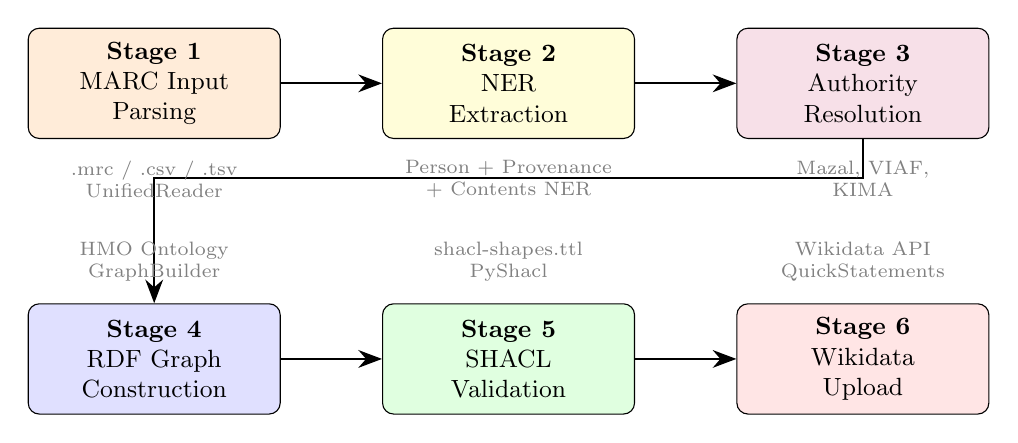
\begin{tikzpicture}[
  stage/.style={draw, rounded corners, minimum height=1.4cm, minimum width=3.2cm,
                align=center, font=\small},
  arrow/.style={-{Stealth[length=3mm]}, thick},
  note/.style={font=\scriptsize, text=gray, align=center},
  >=Stealth
]

\node[stage, fill=orange!15] (input) at (0,0) {\textbf{Stage 1}\\MARC Input\\Parsing};
\node[stage, fill=yellow!15] (ner) at (4.5,0) {\textbf{Stage 2}\\NER\\Extraction};
\node[stage, fill=purple!12] (auth) at (9,0) {\textbf{Stage 3}\\Authority\\Resolution};
\node[stage, fill=blue!12] (rdf) at (0,-3.5) {\textbf{Stage 4}\\RDF Graph\\Construction};
\node[stage, fill=green!12] (valid) at (4.5,-3.5) {\textbf{Stage 5}\\SHACL\\Validation};
\node[stage, fill=red!10] (wiki) at (9,-3.5) {\textbf{Stage 6}\\Wikidata\\Upload};

\draw[arrow] (input) -- (ner);
\draw[arrow] (ner) -- (auth);
\draw[arrow] (auth) -- ++(0,-1.2) -| (rdf);
\draw[arrow] (rdf) -- (valid);
\draw[arrow] (valid) -- (wiki);

\node[note, below=0.15cm of input] {.mrc / .csv / .tsv\\UnifiedReader};
\node[note, below=0.15cm of ner] {Person + Provenance\\+ Contents NER};
\node[note, below=0.15cm of auth] {Mazal, VIAF,\\KIMA};
\node[note, above=0.15cm of rdf] {HMO Ontology\\GraphBuilder};
\node[note, above=0.15cm of valid] {shacl-shapes.ttl\\PyShacl};
\node[note, above=0.15cm of wiki] {Wikidata API\\QuickStatements};

\end{tikzpicture}
\caption{The six-stage MHM MARC-to-RDF-to-Wikidata pipeline.}
\label{fig:pipeline-stages}
\end{figure}

\subsection{Stage Descriptions}

\begin{description}[style=nextline, leftmargin=2cm]
\item[Stage 1: MARC Input Parsing]
  The \code{UnifiedReader} detects the input format (binary MARC \code{.mrc}, CSV, or TSV) and produces a stream of \code{MarcRecord} objects. The \code{field\_handlers.py} module then decomposes each record into an \code{ExtractedData} structure containing typed fields for titles, authors, dates, materials, scripts, notes, contents, provenance, and external identifiers.

\item[Stage 2: NER Extraction]
  Three NER models run sequentially: (1)~the person NER model (\code{JointNERPipeline}) extracts person name spans from note fields (500, 520, 545, 546, 561, 957) and classifies roles using keyword-based heuristics on Hebrew role terms; (2)~the provenance NER model (\code{NERInferencePipeline}) extracts OWNER, DATE, and COLLECTION entities from MARC 561 provenance text; (3)~the contents NER model extracts WORK, FOLIO, and WORK\_AUTHOR entities from MARC 505. All entities are merged into a single list with a \code{source} discriminator (\code{person\_ner}, \code{provenance\_ner}, \code{contents\_ner}).

\item[Stage 3: Authority Resolution]
  Extracted entity names (persons, places, works) are matched against multiple authority sources: the NLI Mazal authority file (local SQLite database with fuzzy matching), VIAF (public SRU API, persons), and KIMA --- an open, attestation-based database of 48,128 Hebrew historical place names, 100\% Wikidata-linked, queried via a local SQLite index. Matched entities receive stable global identifiers.

\item[Stage 4: RDF Graph Construction]
  The \code{GraphBuilder} assembles an RDF graph from the enriched extracted data. The \code{UriGenerator} creates stable URIs for each entity. The builder implements the HMO three-layer architecture: creating F4\_Manifestation\_Singleton instances, Work-Expression pairs, BU-CU-PU composition structures, production and transfer events, text traditions, and epistemological annotations.

\item[Stage 5: SHACL Validation]
  The generated graph is validated against \code{shacl-shapes.ttl} using PyShacl. Violations are reported with severity levels (Violation, Warning, Info) and specific focus nodes, enabling quality assurance before publication.

\item[Stage 6: Wikidata Upload]
  Validated RDF data are transformed into Wikidata statements and uploaded via the Wikidata API and/or QuickStatements. This includes creating and linking Wikidata items for manuscripts, persons, places, and works, with proper qualifiers for dates, sources, and certainty levels.
\end{description}

\subsection{Data Flow Diagram}

\begin{figure}[H]
\centering
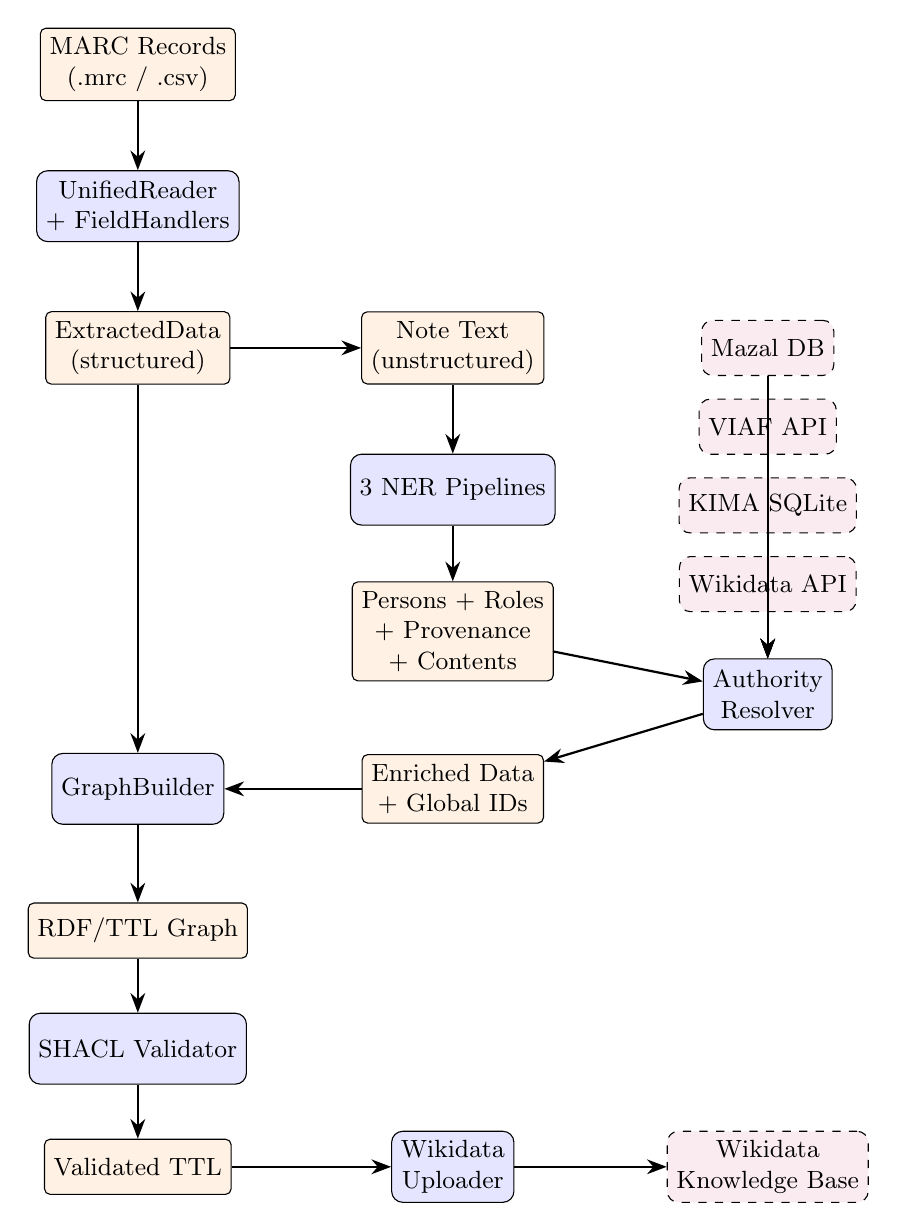
\begin{tikzpicture}[
  data/.style={draw, rounded corners=2pt, fill=orange!10, font=\small, minimum height=0.7cm, align=center},
  proc/.style={draw, rounded corners, fill=blue!10, font=\small, minimum height=0.9cm, align=center},
  ext/.style={draw, dashed, rounded corners, fill=purple!8, font=\small, minimum height=0.7cm, align=center},
  arrow/.style={-{Stealth[length=2.5mm]}, thick},
  >=Stealth
]

\node[data] (marc) at (0,0) {MARC Records\\(.mrc / .csv)};
\node[proc] (parser) at (0,-1.8) {UnifiedReader\\+ FieldHandlers};
\node[data] (extracted) at (0,-3.6) {ExtractedData\\(structured)};
\node[data] (notes) at (4,-3.6) {Note Text\\(unstructured)};
\node[proc] (ner) at (4,-5.4) {3 NER Pipelines};
\node[data] (persons) at (4,-7.2) {Persons + Roles\\+ Provenance\\+ Contents};
\node[ext] (mazal) at (8,-3.6) {Mazal DB};
\node[ext] (viaf) at (8,-4.6) {VIAF API};
\node[ext] (kima) at (8,-5.6) {KIMA SQLite};
\node[ext] (wikidata) at (8,-6.6) {Wikidata API};
\node[proc] (resolver) at (8,-8) {Authority\\Resolver};
\node[data] (enriched) at (4,-9.2) {Enriched Data\\+ Global IDs};
\node[proc] (builder) at (0,-9.2) {GraphBuilder};
\node[data] (rdf) at (0,-11) {RDF/TTL Graph};
\node[proc] (shacl) at (0,-12.5) {SHACL Validator};
\node[data] (output) at (0,-14) {Validated TTL};
\node[proc] (upload) at (4,-14) {Wikidata\\Uploader};
\node[ext] (wd) at (8,-14) {Wikidata\\Knowledge Base};

\draw[arrow] (marc) -- (parser);
\draw[arrow] (parser) -- (extracted);
\draw[arrow] (extracted) -- (notes);
\draw[arrow] (notes) -- (ner);
\draw[arrow] (ner) -- (persons);
\draw[arrow] (mazal) -- (resolver);
\draw[arrow] (viaf) -- (resolver);
\draw[arrow] (kima) -- (resolver);
\draw[arrow] (wikidata) -- (resolver);
\draw[arrow] (persons) -- (resolver);
\draw[arrow] (resolver) -- (enriched);
\draw[arrow] (extracted) -- (builder);
\draw[arrow] (enriched) -- (builder);
\draw[arrow] (builder) -- (rdf);
\draw[arrow] (rdf) -- (shacl);
\draw[arrow] (shacl) -- (output);
\draw[arrow] (output) -- (upload);
\draw[arrow] (upload) -- (wd);

\end{tikzpicture}
\caption{Detailed data flow diagram showing data objects (rounded rectangles), processing components (shaded), and external services (dashed).}
\label{fig:data-flow}
\end{figure}

\subsection{Component Interaction Model}

The pipeline components are implemented as Python modules with well-defined interfaces:

\begin{itemize}
\item \code{converter.parser.unified\_reader.UnifiedReader} --- input abstraction layer
\item \code{converter.transformer.field\_handlers.extract\_all\_data()} --- MARC decomposition
\item \code{converter.transformer.mapper.MarcToRdfMapper} --- orchestrator
\item \code{converter.rdf.graph\_builder.GraphBuilder} --- RDF construction
\item \code{converter.authority.mazal\_matcher.MazalMatcher} --- local authority resolution
\item \code{ner.inference\_pipeline.JointNERPipeline} --- person NER + keyword-based role classification
\item \code{ner.ner\_inference\_pipeline.NERInferencePipeline} --- provenance and contents NER (shared DictaBERT base)
\item \code{converter.validation.shacl\_validator.ShaclValidator} --- constraint checking
\end{itemize}

The \code{MarcToRdfMapper} class serves as the main orchestrator, accepting a \code{MarcRecord} and optionally a \code{MazalMatcher} instance, and coordinating the extraction, enrichment, and graph construction process.


%% ============================================================
%% CHAPTER 4: COMPONENT 1 --- MARC PARSER
%% ============================================================
\section{Component 1: MARC Parser}
\label{sec:marc-parser}

\subsection{UnifiedReader Architecture}

The MARC parser provides a format-agnostic input layer through the \code{UnifiedReader} class, which auto-detects the input format and delegates to the appropriate reader:

\begin{itemize}
\item \textbf{Binary MARC} (\code{.mrc}): Parsed using the \code{pymarc} library via \code{MarcReader}.
\item \textbf{CSV/TSV}: Parsed via \code{CsvReader}, which maps column headers to MARC field tags.
\end{itemize}

The reader produces an iterator of \code{MarcRecord} objects, each encapsulating the control number (field 001), leader, and a list of \code{MarcField} objects with tags, indicators, and subfields.

\begin{lstlisting}[language=Python, caption={UnifiedReader entry point}]
reader = UnifiedReader(Path("data/mrc/test_manuscripts/all_test_manuscripts.mrc"))
total = reader.count_records()
for record in reader.read_file():
    extracted = extract_all_data(record)
    graph = graph_builder.build_graph(extracted, record.control_number)
\end{lstlisting}

\subsection{MarcRecord Data Model}

The internal \code{MarcRecord} dataclass provides:

\begin{itemize}
\item \code{control\_number: str} --- MARC field 001 (NLI system number, e.g., \code{990000623390205171})
\item \code{leader: str} --- 24-character MARC leader
\item \code{fields: List[MarcField]} --- all data fields
\item Methods: \code{get\_field(tag)}, \code{get\_fields(tag)}, \code{get\_subfield(tag, code)}
\end{itemize}

Each \code{MarcField} contains:
\begin{itemize}
\item \code{tag: str} --- three-digit field tag (e.g., ``245'', ``500'')
\item \code{indicators: Tuple[str, str]} --- two indicator characters
\item \code{subfields: Dict[str, List[str]]} --- subfield code to value(s) mapping
\end{itemize}

\subsection{Field Extraction: ExtractedData}

The \code{extract\_all\_data()} function in \code{field\_handlers.py} processes over 30 MARC fields and produces an \code{ExtractedData} instance containing:

\begin{longtable}{|l|l|p{7cm}|}
\hline
\textbf{Field Group} & \textbf{MARC Source} & \textbf{Extracted Attributes} \\
\hline
\endfirsthead
\hline
\textbf{Field Group} & \textbf{MARC Source} & \textbf{Extracted Attributes} \\
\hline
\endhead
\hline
\endfoot
Core bibliographic & 245, 246 & title, subtitle, variant\_titles \\
\hline
Authors/contributors & 100, 700, 800 & authors, contributors (name, role, dates) \\
\hline
Dates & 008, 260/264 & dates (type, value, certainty) \\
\hline
Physical description & 300 & extent (folios), height\_mm, width\_mm \\
\hline
Material & 340 & materials list \\
\hline
Language/script & 008, 546 & languages, script\_type, script\_mode \\
\hline
Notes & 500, 520, 545, 546 & notes list (free text) \\
\hline
Contents & 505 & contents (title, author per entry) \\
\hline
Subjects & 600, 650, 651 & subjects (term, type, authority) \\
\hline
Provenance & 561 & provenance text \\
\hline
Digital access & 856 & digital\_url \\
\hline
External IDs & 001, 035 & external\_ids dict \\
\hline
Colophon & 957 & colophon\_text \\
\hline
Certainty tracking & various & certainty\_levels, attribution\_sources \\
\hline
Codicological & 505, notes & codicological\_units, is\_anthology, is\_multi\_volume \\
\hline
Scribal & notes & scribal\_interventions \\
\hline
Canonical references & notes & canonical\_references, text\_traditions \\
\hline
\end{longtable}

\subsection{Supported MARC Fields}

The parser handles the following MARC fields:

\begin{longtable}{|l|l|p{8cm}|}
\hline
\textbf{Tag} & \textbf{Name} & \textbf{Usage in Pipeline} \\
\hline
\endfirsthead
\hline
\textbf{Tag} & \textbf{Name} & \textbf{Usage in Pipeline} \\
\hline
\endhead
\hline
\endfoot
001 & Control Number & NLI system number; URI generation \\
\hline
008 & Fixed-Length Data & Date type, date values, language code, place of production \\
\hline
035 & System Control Number & Other system identifiers \\
\hline
090/099 & Call Number & Shelf mark, collection identifier \\
\hline
100 & Main Entry (Person) & Primary author/creator; subfields \$a (name), \$d (dates), \$e (relator) \\
\hline
245 & Title Statement & Main title (\$a), subtitle (\$b), responsibility (\$c) \\
\hline
246 & Variant Title & Alternative titles \\
\hline
260/264 & Publication/Production & Place, publisher/producer, date \\
\hline
300 & Physical Description & Extent (\$a), dimensions (\$c) \\
\hline
340 & Physical Medium & Material type \\
\hline
500 & General Note & Free-text notes; NER extraction target \\
\hline
505 & Contents Note & Anthology/multi-work contents; CU decomposition \\
\hline
520 & Summary Note & Abstract/summary; NER extraction target \\
\hline
545 & Biographical Note & Person biographical data; NER extraction target \\
\hline
546 & Language Note & Language and script information; NER extraction target \\
\hline
561 & Ownership/Custody History & Provenance narrative; NER extraction target \\
\hline
600 & Subject (Person) & Subject persons \\
\hline
650 & Subject (Topical) & Subject headings \\
\hline
651 & Subject (Geographic) & Geographic subjects \\
\hline
700 & Added Entry (Person) & Additional persons; subfields \$a, \$d, \$e \\
\hline
800 & Series Added Entry & Series person entries \\
\hline
856 & Electronic Location & Digital facsimile URLs \\
\hline
957 & Local Note (NLI) & Colophon transcription; NER extraction target \\
\hline
\end{longtable}

\subsection{File Inventory: MARC Parser}

\begin{longtable}{|p{11cm}|r|}
\hline
\textbf{File Path} & \textbf{Size} \\
\hline
\endfirsthead
\hline
\textbf{File Path} & \textbf{Size} \\
\hline
\endhead
\hline
\endfoot
\filepath{pipeline/converter/main.py} & 3.5\,KB \\
\hline
\filepath{pipeline/converter/parser/marc\_reader.py} & --- \\
\hline
\filepath{pipeline/converter/parser/csv\_reader.py} & --- \\
\hline
\filepath{pipeline/converter/parser/unified\_reader.py} & --- \\
\hline
\filepath{pipeline/converter/transformer/field\_handlers.py} & $>$40\,KB \\
\hline
\filepath{pipeline/converter/transformer/mapper.py} & --- \\
\hline
\filepath{pipeline/converter/transformer/uri\_generator.py} & --- \\
\hline
\filepath{pipeline/converter/config/namespaces.py} & --- \\
\hline
\filepath{pipeline/converter/config/vocabularies.py} & --- \\
\hline
\end{longtable}


%% ============================================================
%% CHAPTER 5: COMPONENT 2 --- NER EXTRACTION SYSTEM
%% ============================================================
\section{Component 2: NER Extraction System}
\label{sec:ner}

\subsection{Purpose and Scope}

The NER extraction system addresses a fundamental limitation of MARC records: critical information about persons, provenance, and contents associated with manuscripts is often embedded in free-text note fields rather than in structured fields. The system uses three specialised NER models to extract entities from different MARC field types.

\textbf{Input:} Hebrew text from MARC note fields (500, 520, 545, 546, 561, 957) and contents fields (505).\\
\textbf{Output:} Extracted entities with type and role classifications, unified in a single entity list with a \code{source} discriminator.

Example:
\begin{lstlisting}[basicstyle=\ttfamily\small, frame=none, backgroundcolor=\color{white}]
Input (notes):  "Written by Moses ben Jacob"
Output: {"person": "Moses ben Jacob", "role": "AUTHOR", "source": "person_ner"}

Input (561):    "Owned by the Rothschild family, 1890"
Output: {"text": "Rothschild family", "type": "OWNER", "source": "provenance_ner"}
        {"text": "1890", "type": "DATE", "source": "provenance_ner"}

Input (505):    "Moreh Nevukhim / Moses ben Maimon, ff. 1r-45v"
Output: {"text": "Moreh Nevukhim", "type": "WORK", "source": "contents_ner"}
        {"text": "Moses ben Maimon", "type": "WORK_AUTHOR", "source": "contents_ner"}
        {"text": "1r-45v", "type": "FOLIO", "source": "contents_ner"}
\end{lstlisting}

\subsection{Three-Model Architecture}

\begin{figure}[H]
\centering
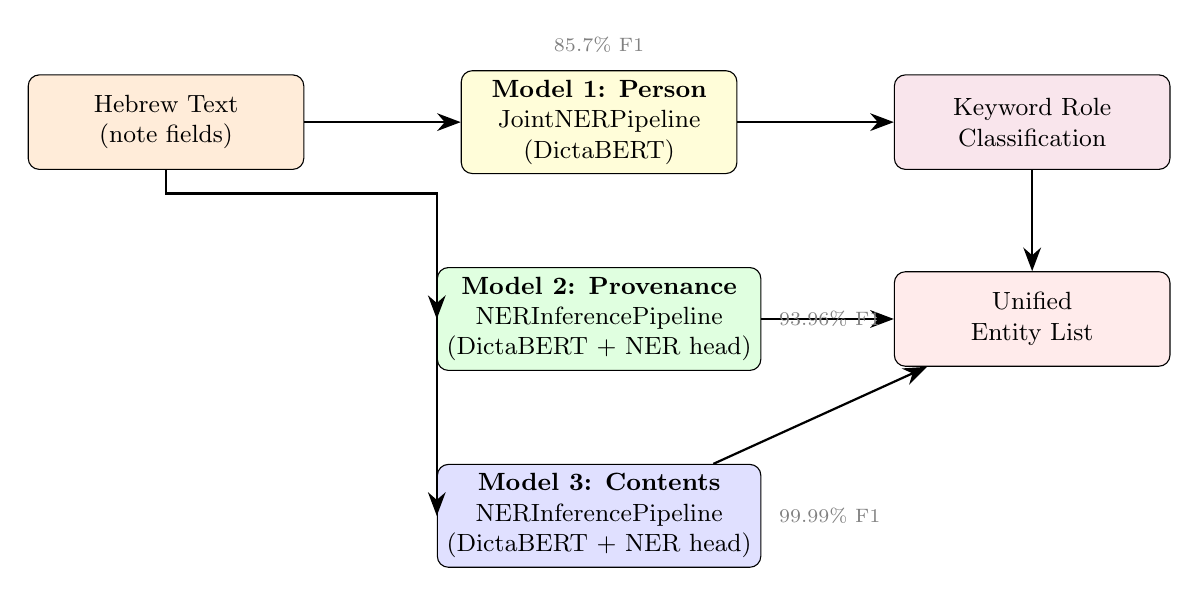
\begin{tikzpicture}[
  box/.style={draw, rounded corners, minimum height=1.2cm, minimum width=3.5cm, align=center, font=\small},
  arrow/.style={-{Stealth[length=3mm]}, thick},
  note/.style={font=\scriptsize, text=gray, align=center},
  >=Stealth
]

\node[box, fill=orange!15] (text) at (0,0) {Hebrew Text\\(note fields)};
\node[box, fill=yellow!15] (person) at (5.5,0) {\textbf{Model 1: Person}\\JointNERPipeline\\(DictaBERT)};
\node[box, fill=green!12] (prov) at (5.5,-2.5) {\textbf{Model 2: Provenance}\\NERInferencePipeline\\(DictaBERT + NER head)};
\node[box, fill=blue!12] (cont) at (5.5,-5) {\textbf{Model 3: Contents}\\NERInferencePipeline\\(DictaBERT + NER head)};
\node[box, fill=purple!10] (merge) at (11,0) {Keyword Role\\Classification};
\node[box, fill=red!8] (out) at (11,-2.5) {Unified\\Entity List};

\draw[arrow] (text) -- (person);
\draw[arrow] (text.south) -- ++(0,-0.3) -| (prov.west);
\draw[arrow] (text.south) -- ++(0,-0.3) -| (cont.west);
\draw[arrow] (person) -- (merge);
\draw[arrow] (merge) -- (out);
\draw[arrow] (prov) -- (out);
\draw[arrow] (cont) -- (out);

\node[note, above=0.1cm of person] {85.7\% F1};
\node[note, right=0.1cm of prov] {93.96\% F1};
\node[note, right=0.1cm of cont] {99.99\% F1};

\end{tikzpicture}
\caption{Three-model NER architecture. Person NER uses keyword-based role classification; provenance and contents models share DictaBERT base.}
\label{fig:ner-architecture}
\end{figure}

\subsubsection{Model 1: Person NER (JointNERPipeline)}

The person NER model is based on DictaBERT, fine-tuned for token classification with BIO labelling (B-PERSON, I-PERSON, O) on a dataset of 7,580 samples derived through distant supervision from 123,621 MARC records.

Key characteristics:
\begin{itemize}
\item Handles 1--10 persons per text segment
\item Multi-entity training improves performance by +2.15\% over single-entity training
\item F1 score: 85.7\% (HuggingFace model: \code{alexgoldberg/hebrew-manuscript-joint-ner-v2})
\end{itemize}

\subsubsection{Role Classification: Keyword-Based Heuristics}

After person NER identifies person name spans, role classification uses keyword-based heuristics on Hebrew role terms in the surrounding context (rather than a separate neural classifier). The \code{\_classify\_role\_by\_keywords()} function detects Hebrew terms associated with each role category. It classifies each person into one of six roles:

\begin{longtable}{|l|p{8cm}|}
\hline
\textbf{Role} & \textbf{Description} \\
\hline
\endfirsthead
\hline
\textbf{Role} & \textbf{Description} \\
\hline
\endhead
\hline
\endfoot
AUTHOR & Creator/composer of the work \\
\hline
TRANSCRIBER & Scribe who copied the manuscript \\
\hline
OWNER & Person who owned or possessed the manuscript \\
\hline
CENSOR & Person who censored the text \\
\hline
TRANSLATOR & Person who translated the work \\
\hline
COMMENTATOR & Person who wrote commentary on the text \\
\hline
\end{longtable}

\subsubsection{Model 2: Provenance NER (NERInferencePipeline)}

The provenance NER model is a DictaBERT base with a single token-classification head, trained on MARC 561 (ownership and custodial history) fields using distant supervision with three extraction strategies: structured cross-referencing, rule-based pattern matching, and Latin censor name identification.

Entity types:
\begin{itemize}
\item \textbf{OWNER} --- person or institution that owned/possessed the manuscript
\item \textbf{DATE} --- dates associated with ownership or provenance events
\item \textbf{COLLECTION} --- named collection or library
\end{itemize}

Training: 10K curated samples from 123K MARC records; 5-fold cross-validation with DictaBERT + NER head; \code{max\_length=64}, \code{batch\_size=32}, \code{lr=3e-5}. F1 score: 93.96\%.

The \code{\_split\_provenance\_text()} function in \code{NerWorker} preprocesses MARC 561 text by splitting on delimiters before inference.

\subsubsection{Model 3: Contents NER (NERInferencePipeline)}

The contents NER model shares the same DictaBERT + NER head architecture, trained on MARC 505 (contents) fields using rule-based parsing of structured contents notes.

Entity types:
\begin{itemize}
\item \textbf{WORK} --- title of a literary work contained in the manuscript
\item \textbf{FOLIO} --- folio range of the work within the manuscript
\item \textbf{WORK\_AUTHOR} --- author of the contained work
\end{itemize}

Training: 10K curated samples (all with WORK+FOLIO+WORK\_AUTHOR triples); same hyperparameters as provenance model. F1 score: 99.99\%.

\subsubsection{Shared DictaBERT Base}

The provenance and contents models share a single DictaBERT base model via \code{NERInferencePipeline.from\_shared\_base()}, reducing memory from $\sim$2.1\,GB (loading DictaBERT three times) to $\sim$700\,MB. Model paths resolve in order: explicit kwarg $\to$ environment variable (\code{MHM\_BUNDLED\_PROVENANCE\_MODEL} / \code{MHM\_BUNDLED\_CONTENTS\_MODEL}) $\to$ repo-relative fallback (\filepath{ner/provenance\_ner\_model.pt}).

\subsubsection{Post-Processing Rules}

The \code{PostProcessingRules} module applies rule-based corrections to person NER output, handling edge cases such as:
\begin{itemize}
\item Merging split name tokens
\item Removing false positive matches (common words misidentified as names)
\item Resolving Hebrew patronymic patterns (``ben'', ``bar'', ``bat'')
\end{itemize}

\subsection{Model Performance Comparison}

\begin{table}[H]
\centering
\begin{tabular}{llrr}
\toprule
\textbf{Task} & \textbf{Model} & \textbf{Score} & \textbf{Training Data} \\
\midrule
Person NER & DictaBERT (baseline) & 80.42\% F1 & General Hebrew \\
Person NER & HalleluBERT (single) & 86.56\% F1 & 8,186 single-person \\
\textbf{Person NER} & \textbf{DictaBERT (multi, v2)} & \textbf{85.7\% F1} & \textbf{7,580 mixed} \\
\midrule
Role & Keyword heuristics & --- & Hebrew role terms \\
\midrule
\textbf{Provenance NER} & \textbf{DictaBERT + NER head} & \textbf{93.96\% F1} & \textbf{10K from 123K MARC} \\
\textbf{Contents NER} & \textbf{DictaBERT + NER head} & \textbf{99.99\% F1} & \textbf{10K from 123K MARC} \\
\bottomrule
\end{tabular}
\caption{NER model comparison across all three pipelines.}
\label{tab:ner-models}
\end{table}

\subsection{Training Data: Distant Supervision}

All three NER models use the same distant supervision methodology (Goldberg, Prebor \& Elmalech 2025):

\textbf{Person NER:} Structured person fields from MARC (100\$a, 600\$a, 700\$a, 800\$a) were matched against concatenated note fields (500\$a, 520\$a, 545\$a, 546\$a, 561\$a, 957\$a) using fuzzy string matching.

\textbf{Provenance NER:} Three extraction strategies from MARC 561: structured cross-referencing against authority fields, rule-based pattern matching for ownership phrases, and Latin censor name identification. Produced 10K curated samples from 123K records.

\textbf{Contents NER:} Rule-based parsing of MARC 505 structured contents notes (title / author / folio triples). Produced 10K curated samples, all containing WORK+FOLIO+WORK\_AUTHOR.

\begin{table}[H]
\centering
\begin{tabular}{lrrr}
\toprule
\textbf{Dataset} & \textbf{Train} & \textbf{Val} & \textbf{Test} \\
\midrule
Person NER (multi-entity, filtered) & 6,058 & 757 & 765 \\
Provenance NER & 8,000 & 1,000 & 1,000 \\
Contents NER & 8,000 & 1,000 & 1,000 \\
K-fold (5 folds, each model) & \multicolumn{3}{c}{5 $\times$ train/val splits} \\
\bottomrule
\end{tabular}
\caption{NER training dataset splits for all three models.}
\label{tab:ner-data}
\end{table}

Person NER dataset composition: 85.4\% single-person samples, 10.1\% multi-person (639 with 2 persons, 152 with 3, 32 with 4+).

\subsection{MARC Fields Targeted by NER}

\begin{longtable}{|l|l|p{5cm}|l|}
\hline
\textbf{MARC Field} & \textbf{Subfield} & \textbf{Content Type} & \textbf{NER Model} \\
\hline
\endfirsthead
\hline
\textbf{MARC Field} & \textbf{Subfield} & \textbf{Content Type} & \textbf{NER Model} \\
\hline
\endhead
\hline
\endfoot
500 & \$a & General notes & Person NER \\
\hline
505 & \$a & Formatted contents note & Contents NER \\
\hline
520 & \$a & Summary/abstract notes & Person NER \\
\hline
545 & \$a & Biographical or historical notes & Person NER \\
\hline
546 & \$a & Language notes & Person NER \\
\hline
561 & \$a & Ownership and custodial history & Provenance NER \\
\hline
957 & \$a & Local NLI colophon transcription & Person NER \\
\hline
\end{longtable}

\subsection{Integration Point}

The NER system is invoked through three pipeline classes, orchestrated by \code{NerWorker}:

\begin{lstlisting}[language=Python, caption={Three-model NER pipeline invocation}]
from ner.inference_pipeline import JointNERPipeline
from ner.ner_inference_pipeline import NERInferencePipeline

# Model 1: Person NER (keyword-based role classification)
person_pipeline = JointNERPipeline(model_path="alexgoldberg/hebrew-manuscript-joint-ner-v2")
person_results = person_pipeline.process(text)
# Returns: [{"person": "name", "role": "AUTHOR", "source": "person_ner"}]

# Models 2+3: Provenance + Contents NER (shared DictaBERT base)
prov_pipeline = NERInferencePipeline(model_path="ner/provenance_ner_model.pt")
cont_pipeline = NERInferencePipeline.from_shared_base(
    prov_pipeline, model_path="ner/contents_ner_model.pt"
)
prov_results = prov_pipeline.predict(provenance_text)
# Returns: [{"text": "Owner", "type": "OWNER", "source": "provenance_ner"}]
cont_results = cont_pipeline.predict(contents_text)
# Returns: [{"text": "Title", "type": "WORK", "source": "contents_ner"}]
\end{lstlisting}

\subsection{File Inventory: NER System}

\begin{longtable}{|p{10cm}|r|}
\hline
\textbf{File Path} & \textbf{Size} \\
\hline
\endfirsthead
\hline
\textbf{File Path} & \textbf{Size} \\
\hline
\endhead
\hline
\endfoot
\filepath{pipeline/ner/inference\_pipeline.py} & --- \\
\hline
\filepath{pipeline/ner/ner\_inference\_pipeline.py} & --- \\
\hline
\filepath{pipeline/ner/postprocessing\_rules.py} & --- \\
\hline
\filepath{pipeline/ner/extract\_marc\_entities.py} & --- \\
\hline
\filepath{pipeline/ner/extract\_provenance\_entities.py} & --- \\
\hline
\filepath{pipeline/ner/extract\_contents\_entities.py} & --- \\
\hline
\filepath{pipeline/ner/extract\_multi\_entity\_dataset.py} & --- \\
\hline
\filepath{pipeline/ner/train\_ner\_model\_kfold.py} & --- \\
\hline
\filepath{pipeline/ner/train\_joint\_entity\_role\_model.py} & --- \\
\hline
\filepath{pipeline/ner/train\_joint\_entity\_role\_model\_kfold.py} & --- \\
\hline
\filepath{pipeline/ner/joint\_entity\_role\_model/best\_model.pt} & 2.1\,GB \\
\hline
\filepath{pipeline/ner/provenance\_ner\_model.pt} & 704\,MB \\
\hline
\filepath{pipeline/ner/contents\_ner\_model.pt} & 704\,MB \\
\hline
\filepath{pipeline/ner/joint\_entity\_role\_model\_kfold/fold\_1\_model.pt} & 706\,MB \\
\hline
\filepath{pipeline/ner/joint\_entity\_role\_model\_kfold/fold\_2\_model.pt} & 706\,MB \\
\hline
\filepath{pipeline/ner/joint\_entity\_role\_model\_kfold/fold\_3\_model.pt} & 706\,MB \\
\hline
\filepath{pipeline/ner/joint\_entity\_role\_model\_kfold/fold\_4\_model.pt} & 706\,MB \\
\hline
\filepath{pipeline/ner/joint\_entity\_role\_model\_kfold/fold\_5\_model.pt} & 706\,MB \\
\hline
\filepath{pipeline/ner/raw-data/full-data.csv} & 1.1\,GB \\
\hline
\filepath{pipeline/ner/processed-data/} (74 files) & various \\
\hline
\end{longtable}


%% ============================================================
%% CHAPTER 6: COMPONENT 3 --- AUTHORITY FILE INTEGRATION
%% ============================================================
\section{Component 3: Authority File Integration}
\label{sec:authority}

\subsection{Overview}

Authority file integration is the stage where extracted entity names---whether from structured MARC fields or from NER output---are matched against authoritative external databases to obtain unique, globally recognised identifiers. This process serves three purposes:

\begin{enumerate}
\item \textbf{Disambiguation:} Resolving multiple name variants (``Maimonides'', ``Rambam'', ``Moses ben Maimon'') to a single canonical entity.
\item \textbf{Enrichment:} Adding external identifiers (VIAF ID, NLI ID, Wikidata QID) that enable cross-repository linking.
\item \textbf{Validation:} Confirming that cataloged names correspond to known historical persons, places, or works.
\end{enumerate}

\subsection{NLI Authority File (Mazal)}

The primary authority source is the NLI's own authority file, locally indexed in a SQLite database referred to as the ``Mazal index'' (after the Hebrew-language system name).

\subsubsection{Architecture}

The authority matching system consists of two classes:

\begin{itemize}
\item \code{MazalIndex} (\filepath{converter/authority/mazal\_index.py}): Low-level SQLite interface providing lookup methods for persons, places, works, and corporate bodies.
\item \code{MazalMatcher} (\filepath{converter/authority/mazal\_matcher.py}): High-level service wrapper providing fuzzy matching, statistics tracking, and configurable fallback behaviour.
\end{itemize}

\subsubsection{Entity Types Supported}

\begin{longtable}{|l|l|p{6cm}|}
\hline
\textbf{Entity Type} & \textbf{Method} & \textbf{Parameters} \\
\hline
\endfirsthead
\hline
\textbf{Entity Type} & \textbf{Method} & \textbf{Parameters} \\
\hline
\endhead
\hline
\endfoot
Person & \code{match\_person()} & name (Hebrew/Latin), optional dates \\
\hline
Place & \code{match\_place()} & place name (Hebrew/Latin) \\
\hline
Work & \code{match\_work()} & title, optional author \\
\hline
Corporate body & \code{match\_corporate()} & organisation name \\
\hline
\end{longtable}

\subsubsection{Matching Process}

The matcher attempts exact matching first, then falls back to fuzzy matching for near-variants. Statistics are tracked per entity type:

\begin{lstlisting}[language=Python, caption={Authority matching usage}]
from converter.authority.mazal_matcher import MazalMatcher

with MazalMatcher() as matcher:
    nli_id = matcher.match_person("Gikatilla, Joseph ben Abraham", 
                                   dates="1248-1305")
    place_id = matcher.match_place("Candia")
    work_id = matcher.match_work("Ginat Egoz")
    
    stats = matcher.get_stats()
    print(matcher.get_unmatched_summary())
\end{lstlisting}

\subsubsection{Database}

The Mazal index database is stored at \filepath{pipeline/converter/authority/mazal\_index.db} (983\,MB). It contains records for persons, places, works, and corporate bodies extracted from the NLI authority file system.

\subsection{VIAF Integration (Planned)}

The Virtual International Authority File (VIAF) aggregates authority records from national libraries worldwide. VIAF integration will use the VIAF API to:

\begin{itemize}
\item Search for person and corporate body records by name
\item Retrieve VIAF cluster IDs for matched entities
\item Access cross-references to national authority files (Library of Congress, BnF, DNB, etc.)
\end{itemize}

The VIAF API endpoint (\code{https://viaf.org/viaf/search}) supports SRU (Search/Retrieve via URL) queries with CQL (Contextual Query Language).

\subsection{Library of Congress Name Authority File (Planned)}

The Library of Congress Name Authority File (LCNAF) will be queried via the LC Linked Data Service API (\code{https://id.loc.gov/}) to:

\begin{itemize}
\item Verify name headings against the world's largest English-language authority file
\item Obtain LC authority identifiers for cross-referencing
\item Access alternative name forms and biographical data
\end{itemize}

\subsection{KIMA Hebrew Place Names (Implemented)}

Geographic names---production places, ownership locations, current repositories---are enriched through KIMA (\texthebrew{קימ"א}, \emph{Corpus of Hebrew Place Name Attestations}), an open, attestation-based database maintained by HLT/INT and the National Library of Israel.

KIMA covers 48,128 historical Hebrew-script place names with:
\begin{itemize}
\item 100\% Wikidata linkage (every record has a \code{Q}-identifier)
\item VIAF and GeoNames identifiers stored as cross-references (no external API calls)
\item 48,225 Hebrew name variants and Maagarim grammatical word-forms for morphological matching
\end{itemize}

The integration uses a local SQLite index (\filepath{data/kima/kima\_index.db}) built from three TSV source files:
\begin{itemize}
\item \filepath{20251015 Kima places.tsv} --- 48,128 primary place records with coordinates
\item \filepath{Kima-Hebrew-Variants-20250929.tsv} --- 48,225 Hebrew name variants
\item \filepath{Maagarim-Zurot-\&-Arachim.tsv} --- 14,522 grammatical word-forms (inflected/suffixed forms)
\end{itemize}

The \code{KimaIndex} normalises queries by stripping Hebrew niqqud, diacritics, and parenthetical geopolitical context (e.g.\ \texthebrew{ישראל} in \texthebrew{ירושלים (ישראל)}), then performs exact lookup against the indexed forms. A match returns the Wikidata URI, with VIAF as fallback.

\subsection{Resolution Strategy}

Authority resolution follows a cascading priority by entity type:

\textbf{Persons (NER-extracted):}
\begin{enumerate}
\item \textbf{Local (Mazal):} Query the NLI authority file first (fastest, domain-specific).
\item \textbf{VIAF:} If no Mazal match, query VIAF via the public SRU API (no API key required).
\item \textbf{Unresolved:} Entity flagged with name only; manual review.
\end{enumerate}

\textbf{Places (from MARC fields):}
\begin{enumerate}
\item \textbf{KIMA:} Query the local KIMA SQLite index (48k Hebrew historical place names, 100\% Wikidata-linked).
\item \textbf{Unresolved:} Place stored as literal; manual review.
\end{enumerate}

\subsection{File Inventory: Authority Integration}

\begin{longtable}{|p{10cm}|r|}
\hline
\textbf{File Path} & \textbf{Size} \\
\hline
\endfirsthead
\hline
\textbf{File Path} & \textbf{Size} \\
\hline
\endhead
\hline
\endfoot
\filepath{pipeline/converter/authority/mazal\_index.py} & --- \\
\hline
\filepath{pipeline/converter/authority/mazal\_matcher.py} & --- \\
\hline
\filepath{pipeline/converter/authority/mazal\_index.db} & 983\,MB \\
\hline
\filepath{pipeline/converter/authority/kima\_index.py} & --- \\
\hline
\filepath{pipeline/converter/authority/kima\_matcher.py} & --- \\
\hline
\filepath{pipeline/data/kima/kima\_index.db} & $\sim$25\,MB \\
\hline
\filepath{pipeline/data/kima/20251015 Kima places.tsv} & --- \\
\hline
\filepath{pipeline/data/kima/Kima-Hebrew-Variants-20250929.tsv} & --- \\
\hline
\filepath{pipeline/data/kima/Maagarim-Zurot-\&-Arachim.tsv} & --- \\
\hline
\end{longtable}


%% ============================================================
%% CHAPTER 7: COMPONENT 4 --- RDF GRAPH BUILDER
%% ============================================================
\section{Component 4: RDF Graph Builder}
\label{sec:rdf-builder}

\subsection{HMO Ontology Structure}

The RDF Graph Builder constructs an RDF/OWL graph conforming to the Hebrew Manuscripts Ontology (HMO). The ontology is defined in \filepath{pipeline/ontology/hebrew-manuscripts.ttl} (143\,KB) with controlled vocabularies in \filepath{pipeline/ontology/controlled-vocabularies.ttl} (29\,KB).

HMO implements a three-layer architecture:

\subsubsection{Cataloging-Bibliographic Layer}

This layer represents manuscripts using the LRMoo/CIDOC CRM entity hierarchy:

\begin{itemize}
\item \code{lrmoo:F1\_Work} --- abstract intellectual creation
\item \code{lrmoo:F2\_Expression} --- specific textual realisation
\item \code{lrmoo:F4\_Manifestation\_Singleton} --- unique physical manuscript (retained from FRBRoo despite deprecation in LRMoo, as a pragmatic modelling choice)
\item \code{cidoc-crm:E21\_Person} --- persons (authors, scribes, owners)
\item \code{cidoc-crm:E53\_Place} --- geographic locations
\item \code{cidoc-crm:E52\_Time-Span} --- temporal references
\end{itemize}

\subsubsection{Philological Layer}

\begin{itemize}
\item \code{hm:TextTradition} --- a line of textual transmission
\item \code{hm:TransmissionWitness} --- a specific manuscript as witness to a text tradition
\end{itemize}

\subsubsection{Epistemological Layer}

\begin{itemize}
\item \code{hm:Attribution} --- links a claim to its source (colophon, catalog, scholarship)
\item \code{hm:EpistemologicalStatus} --- certainty level (certain, probable, conjectured)
\end{itemize}

\subsection{BU-CU-PU Structural Model}

Physical manuscript structure is represented through composition relationships:

\begin{itemize}
\item \textbf{Bibliographic Unit (BU):} The entire physical volume under a single shelf mark.
\item \textbf{Codicological Unit (CU):} A distinct part created at a specific time and place.
\item \textbf{Paleographical Unit (PU):} A part written by a specific scribal hand.
\end{itemize}

Relationships: \code{hm:is\_composed\_of} (BU $\to$ CU, CU $\to$ PU) and \code{hm:forms\_part\_of} (inverse).

\subsection{Event-Centric Modelling}

The graph builder creates event nodes for:

\begin{itemize}
\item \code{cidoc-crm:E12\_Production} --- manuscript copying events, linked to scribe (Person), place, and date
\item \code{lrmoo:F28\_Expression\_Creation} --- creation of specific textual expression
\item \code{cidoc-crm:E8\_Acquisition} --- ownership acquisition events
\item \code{cidoc-crm:E10\_Transfer\_of\_Custody} --- custody transfer events
\end{itemize}

Each event links objects, persons, places, and time spans, enabling queries such as ``all manuscripts copied in Candia in the fifteenth century.''

\subsection{URI Generation}

The \code{UriGenerator} class creates deterministic URIs based on:

\begin{itemize}
\item Manuscripts: \code{hm:MS\_\{control\_number\}}
\item Persons: \code{hm:Person\_\{normalised\_name\}} or \code{hm:Person\_\{nli\_id\}} when authority-matched
\item Places: \code{hm:Place\_\{normalised\_name\}}
\item Works: \code{hm:Work\_\{control\_number\}\_\{index\}}
\item Events: \code{hm:Production\_\{control\_number\}}, \code{hm:Acquisition\_\{control\_number\}}
\end{itemize}

When a \code{MazalMatcher} is provided, the URI generator attempts to resolve names to NLI authority IDs, producing more stable and reusable URIs.

\subsection{Graph Serialisation}

The completed graph is serialised to Turtle format using \code{rdflib}'s serialiser, with namespace bindings defined in \code{namespaces.py}:

\begin{lstlisting}[language=Python, caption={Graph serialisation}]
combined_graph.serialize(destination="output.ttl", format='turtle')
\end{lstlisting}

\subsection{LOD Integration Properties}

The graph builder generates the following LOD integration triples at the schema level:

\begin{itemize}
\item \code{owl:equivalentProperty} declarations linking HMO properties to Wikidata properties (e.g., \code{has\_number\_of\_folios} $\equiv$ P792)
\item \code{owl:sameAs} placeholders for entity-level linking
\item External identifier properties: \code{viaf\_id}, \code{wikidata\_id}, \code{external\_identifier\_nli}
\end{itemize}

\subsection{File Inventory: RDF Graph Builder}

\begin{longtable}{|p{10cm}|r|}
\hline
\textbf{File Path} & \textbf{Size} \\
\hline
\endfirsthead
\hline
\textbf{File Path} & \textbf{Size} \\
\hline
\endhead
\hline
\endfoot
\filepath{pipeline/converter/rdf/graph\_builder.py} & --- \\
\hline
\filepath{pipeline/converter/rdf/serializer.py} & --- \\
\hline
\filepath{pipeline/converter/transformer/uri\_generator.py} & --- \\
\hline
\filepath{pipeline/converter/config/namespaces.py} & --- \\
\hline
\filepath{pipeline/ontology/hebrew-manuscripts.ttl} & 143\,KB \\
\hline
\filepath{pipeline/ontology/controlled-vocabularies.ttl} & 29\,KB \\
\hline
\filepath{pipeline/ontology/hebrew-manuscripts-original.ttl} & 122\,KB \\
\hline
\end{longtable}


%% ============================================================
%% CHAPTER 8: COMPONENT 5 --- SHACL VALIDATION
%% ============================================================
\section{Component 5: SHACL Validation}
\label{sec:shacl}

\subsection{Purpose}

SHACL (Shapes Constraint Language) validation ensures that the generated RDF graph conforms to the expected structure defined by the HMO ontology. The validation layer catches errors such as missing required properties, incorrect data types, invalid cardinalities, and orphaned nodes.

\subsection{SHACL Shapes}

The shapes are defined in \filepath{pipeline/ontology/shacl-shapes.ttl} (31\,KB). Key shape definitions include:

\begin{itemize}
\item \textbf{ManuscriptShape:} Validates that each F4\_Manifestation\_Singleton has required properties (title, control number, at least one material, language).
\item \textbf{PersonShape:} Validates that E21\_Person entities have labels and optional date/role properties.
\item \textbf{ProductionEventShape:} Validates that E12\_Production events link to at least one person and optionally to a place and time span.
\item \textbf{CodicologicalUnitShape:} Validates BU-CU-PU composition relationships.
\item \textbf{WorkExpressionShape:} Validates Work-Expression-Manifestation chains.
\end{itemize}

\subsection{ShaclValidator Implementation}

The \code{ShaclValidator} class wraps the PyShacl library:

\begin{lstlisting}[language=Python, caption={SHACL validation}]
from converter.validation.shacl_validator import ShaclValidator

validator = ShaclValidator()
result = validator.validate(combined_graph)

if result.conforms:
    print("Validation passed!")
else:
    print(f"Found {result.violation_count} issues:")
    for v in result.violations:
        print(f"  [{v.severity}] {v.focus_node}: {v.message}")
\end{lstlisting}

The validator loads the SHACL shapes graph from the ontology directory and validates the data graph against it. Results include:

\begin{itemize}
\item \code{conforms: bool} --- whether the graph passes all constraints
\item \code{violation\_count: int} --- total number of violations
\item \code{violations: List} --- detailed violation objects with severity, focus node, source shape, path, and message
\end{itemize}

\subsection{Validation Report}

Previous validation runs on the 10,000-record subset produced a validation report stored at \filepath{pipeline/data/marc-subset-10k.validation-report.md}, documenting common violation patterns and their causes.

\subsection{File Inventory: SHACL Validation}

\begin{longtable}{|p{10cm}|r|}
\hline
\textbf{File Path} & \textbf{Size} \\
\hline
\endfirsthead
\hline
\textbf{File Path} & \textbf{Size} \\
\hline
\endhead
\hline
\endfoot
\filepath{pipeline/ontology/shacl-shapes.ttl} & 31\,KB \\
\hline
\filepath{pipeline/converter/validation/shacl\_validator.py} & --- \\
\hline
\filepath{pipeline/data/marc-subset-10k.validation-report.md} & --- \\
\hline
\end{longtable}


%% ============================================================
%% CHAPTER 9: MARC-TO-HMO FIELD MAPPING CROSSWALK
%% ============================================================
\section{MARC-to-HMO Field Mapping Crosswalk}
\label{sec:crosswalk}

\subsection{Mapping Principles}

The MARC-to-HMO crosswalk follows five core principles:

\begin{enumerate}
\item \textbf{WEMI Model:} MARC records map primarily to F4\_Manifestation\_Singleton.
\item \textbf{Works and Expressions:} Derived from content analysis (fields 505, 700).
\item \textbf{Events:} Production and ownership transfers represented as CIDOC CRM events.
\item \textbf{Controlled Vocabularies:} Use existing HMO controlled vocabulary instances for materials, scripts, languages.
\item \textbf{External Links:} Preserve NLI identifiers for future reconciliation.
\end{enumerate}

\subsection{Core Entity Mapping}

\begin{longtable}{|l|l|l|p{5cm}|}
\hline
\textbf{MARC} & \textbf{Subfield} & \textbf{HMO Property} & \textbf{Notes} \\
\hline
\endfirsthead
\hline
\textbf{MARC} & \textbf{Subfield} & \textbf{HMO Property} & \textbf{Notes} \\
\hline
\endhead
\hline
\endfoot
001 & --- & \code{hm:external\_identifier\_nli} & Control number \\
\hline
035 & \$a & \code{cidoc:P1\_is\_identified\_by} & Other identifiers \\
\hline
090/099 & \$a & \code{rdfs:label} & Call number \\
\hline
008[35-37] & --- & \code{hm:has\_language} & Language code \\
\hline
008[06-14] & --- & \code{hm:has\_production\_date} & Date type + values \\
\hline
100 & \$a, \$d, \$e & \code{hm:has\_author} / Person & Main entry \\
\hline
245 & \$a, \$b & \code{hm:has\_title} & Title, subtitle \\
\hline
300 & \$a & \code{hm:has\_number\_of\_folios} & Extent \\
\hline
300 & \$c & \code{hm:has\_height\_mm} & Dimensions \\
\hline
340 & \$a & \code{hm:has\_material} & Material type \\
\hline
505 & \$a, \$r & Work/Expression pairs & Contents note \\
\hline
561 & \$a & Provenance events & Ownership history \\
\hline
700 & \$a, \$d, \$e & \code{hm:has\_scribe} etc. & Added person \\
\hline
856 & \$u & \code{hm:has\_digital\_url} & Digital access \\
\hline
957 & \$a & \code{hm:has\_colophon\_text} & Colophon \\
\hline
\end{longtable}

\subsection{Wikidata Property Alignments}

\begin{longtable}{|l|l|l|}
\hline
\textbf{HMO Property} & \textbf{Wikidata Property} & \textbf{Alignment} \\
\hline
\endfirsthead
\hline
\textbf{HMO Property} & \textbf{Wikidata Property} & \textbf{Alignment} \\
\hline
\endhead
\hline
\endfoot
\code{hm:has\_number\_of\_folios} & P792 & \code{owl:equivalentProperty} \\
\hline
\code{hm:has\_material} & P186 & \code{owl:equivalentProperty} \\
\hline
\code{hm:has\_script\_type} & P6573 & \code{owl:equivalentProperty} \\
\hline
\code{hm:external\_identifier\_nli} & P8189 & \code{owl:equivalentProperty} \\
\hline
\code{hm:has\_viaf\_id} & P214 & \code{owl:equivalentProperty} \\
\hline
\code{hm:has\_wikidata\_id} & --- & \code{owl:sameAs} target \\
\hline
\end{longtable}

\subsection{Detailed Mapping Documentation}

The complete field-by-field mapping is documented in:
\begin{itemize}
\item \filepath{pipeline/mappings/marc-to-rdf-mapping.md} (narrative documentation with RDF patterns)
\item \filepath{pipeline/mappings/marc-mapping-table.csv} (tabular reference)
\end{itemize}


%% ============================================================
%% CHAPTER 10: DATA INVENTORY
%% ============================================================
\section{Data Inventory}
\label{sec:inventory}

This chapter provides a complete inventory of all data files, model artifacts, and ontology definitions in the pipeline repository.

\subsection{Source MARC Data}

\begin{longtable}{|p{9cm}|r|p{3cm}|}
\hline
\textbf{File Path} & \textbf{Size} & \textbf{Description} \\
\hline
\endfirsthead
\hline
\textbf{File Path} & \textbf{Size} & \textbf{Description} \\
\hline
\endhead
\hline
\endfoot
\filepath{pipeline/data/mrc/BIBLIOGRAPHIC\_50929717600005171\_3.mrc} & 229\,MB & Full NLI catalog dump ($\sim$50,929 records) \\
\hline
\filepath{pipeline/data/mrc/test\_manuscripts/all\_test\_manuscripts.mrc} & 25\,KB & Combined 6 pilot manuscripts \\
\hline
\filepath{pipeline/data/mrc/test\_manuscripts/990000623390205171.mrc} & 4.3\,KB & Barberini Or.\ 82 \\
\hline
\filepath{pipeline/data/mrc/test\_manuscripts/990000836520205171.mrc} & 5.9\,KB & Vatican Ebr.\ 44 \\
\hline
\filepath{pipeline/data/mrc/test\_manuscripts/990000991020205171.mrc} & 4.0\,KB & Parma 3122 \\
\hline
\filepath{pipeline/data/mrc/test\_manuscripts/990000993900205171.mrc} & 3.6\,KB & Huntington 115 \\
\hline
\filepath{pipeline/data/mrc/test\_manuscripts/990001967550205171.mrc} & 5.0\,KB & Oppenheimer 129 \\
\hline
\filepath{pipeline/data/mrc/test\_manuscripts/990033752260205171.mrc} & 2.7\,KB & Jerusalem 8210 \\
\hline
\end{longtable}

\subsection{RDF Output Data}

\begin{longtable}{|p{9cm}|r|p{3cm}|}
\hline
\textbf{File Path} & \textbf{Size} & \textbf{Description} \\
\hline
\endfirsthead
\hline
\textbf{File Path} & \textbf{Size} & \textbf{Description} \\
\hline
\endhead
\hline
\endfoot
\filepath{pipeline/data/output/test\_manuscripts\_merged.ttl} & 295\,KB & 6 pilot manuscripts (merged with ontology) \\
\hline
\filepath{pipeline/data/output/test\_manuscripts.ttl} & 165\,KB & 6 pilot manuscripts (data only) \\
\hline
\filepath{pipeline/data/output/old\_test\_manuscripts.ttl} & 161\,KB & Previous version \\
\hline
\filepath{pipeline/data/output/17th\_century\_samples.ttl} & 2.0\,MB & 17th-century subset \\
\hline
\filepath{pipeline/data/output/father\_entities\_100.ttl} & 452\,KB & 100-record sample \\
\hline
\filepath{pipeline/data/output/father\_entities\_sample.ttl} & 378\,KB & Entity sample \\
\hline
\filepath{pipeline/data/output/nli\_sample\_100.ttl} & 111\,KB & 100-record NLI sample \\
\hline
\filepath{pipeline/data/output/csv\_sample.ttl} & 8.5\,KB & CSV conversion test \\
\hline
\filepath{pipeline/data/pilot-sample/sample-barberini-82.ttl} & --- & Individual pilot \\
\hline
\end{longtable}

\subsection{Ontology Files}

\begin{longtable}{|p{9cm}|r|p{3cm}|}
\hline
\textbf{File Path} & \textbf{Size} & \textbf{Description} \\
\hline
\endfirsthead
\hline
\textbf{File Path} & \textbf{Size} & \textbf{Description} \\
\hline
\endhead
\hline
\endfoot
\filepath{pipeline/ontology/hebrew-manuscripts.ttl} & 143\,KB & HMO ontology (current) \\
\hline
\filepath{pipeline/ontology/hebrew-manuscripts-original.ttl} & 122\,KB & HMO ontology (original) \\
\hline
\filepath{pipeline/ontology/controlled-vocabularies.ttl} & 29\,KB & Controlled vocabularies \\
\hline
\filepath{pipeline/ontology/shacl-shapes.ttl} & 31\,KB & SHACL validation shapes \\
\hline
\filepath{pipeline/ontology/catalog-v001.xml} & 265\,B & Prot\'{e}g\'{e} catalog \\
\hline
\end{longtable}

\subsection{NER Model Checkpoints}

\begin{longtable}{|p{9cm}|r|p{3cm}|}
\hline
\textbf{File Path} & \textbf{Size} & \textbf{Description} \\
\hline
\endfirsthead
\hline
\textbf{File Path} & \textbf{Size} & \textbf{Description} \\
\hline
\endhead
\hline
\endfoot
\filepath{pipeline/ner/joint\_entity\_role\_model/best\_model.pt} & 2.1\,GB & Person NER model (joint) \\
\hline
\filepath{pipeline/ner/provenance\_ner\_model.pt} & 704\,MB & Provenance NER model (OWNER/DATE/COLLECTION, 93.96\% F1) \\
\hline
\filepath{pipeline/ner/contents\_ner\_model.pt} & 704\,MB & Contents NER model (WORK/FOLIO/WORK\_AUTHOR, 99.99\% F1) \\
\hline
\filepath{pipeline/ner/joint\_entity\_role\_model\_kfold/fold\_1\_model.pt} & 706\,MB & K-fold model (fold 1) \\
\hline
\filepath{pipeline/ner/joint\_entity\_role\_model\_kfold/fold\_2\_model.pt} & 706\,MB & K-fold model (fold 2) \\
\hline
\filepath{pipeline/ner/joint\_entity\_role\_model\_kfold/fold\_3\_model.pt} & 706\,MB & K-fold model (fold 3) \\
\hline
\filepath{pipeline/ner/joint\_entity\_role\_model\_kfold/fold\_4\_model.pt} & 706\,MB & K-fold model (fold 4) \\
\hline
\filepath{pipeline/ner/joint\_entity\_role\_model\_kfold/fold\_5\_model.pt} & 706\,MB & K-fold model (fold 5) \\
\hline
\filepath{pipeline/ner/joint\_entity\_role\_model\_kfold/kfold\_results.json} & --- & K-fold evaluation results \\
\hline
\end{longtable}

\subsection{NER Training and Evaluation Data}

\begin{longtable}{|p{9cm}|p{4cm}|}
\hline
\textbf{File Path} & \textbf{Description} \\
\hline
\endfirsthead
\hline
\textbf{File Path} & \textbf{Description} \\
\hline
\endhead
\hline
\endfoot
\filepath{pipeline/ner/raw-data/full-data.csv} (1.1\,GB) & Full MARC export (123,621 records) \\
\hline
\filepath{pipeline/ner/processed-data/filtered\_data.csv} & Filtered records with context \\
\hline
\filepath{pipeline/ner/processed-data/top\_10000\_entities.csv} & Top 10,000 by context length \\
\hline
\filepath{pipeline/ner/processed-data/marc\_ner\_train.jsonl} & NER training data (BIO) \\
\hline
\filepath{pipeline/ner/processed-data/marc\_ner\_val.jsonl} & NER validation data \\
\hline
\filepath{pipeline/ner/processed-data/marc\_ner\_test.jsonl} & NER test data \\
\hline
\filepath{pipeline/ner/processed-data/multi\_entity\_train\_filtered.jsonl} & Multi-entity NER train (6,058) \\
\hline
\filepath{pipeline/ner/processed-data/multi\_entity\_val\_filtered.jsonl} & Multi-entity NER val (757) \\
\hline
\filepath{pipeline/ner/processed-data/multi\_entity\_test\_filtered.jsonl} & Multi-entity NER test (765) \\
\hline
\filepath{pipeline/ner/processed-data/role\_classification\_6class\_train.jsonl} & Role classification train \\
\hline
\filepath{pipeline/ner/processed-data/role\_classification\_6class\_val.jsonl} & Role classification val \\
\hline
\filepath{pipeline/ner/processed-data/role\_classification\_6class\_test.jsonl} & Role classification test \\
\hline
\filepath{pipeline/ner/processed-data/kfold/fold\_\{0..4\}\_train.jsonl} & K-fold training splits \\
\hline
\filepath{pipeline/ner/processed-data/kfold/fold\_\{0..4\}\_val.jsonl} & K-fold validation splits \\
\hline
\filepath{pipeline/ner/processed-data/entity\_mappings\_validated.json} & Validated entity mappings \\
\hline
\filepath{pipeline/ner/processed-data/relator\_consolidation\_mapping.json} & Role label mapping \\
\hline
\filepath{pipeline/ner/processed-data/hallelubert\_training\_data\_balanced.json} & Balanced training set \\
\hline
\filepath{pipeline/ner/processed-data/ner\_training\_validated.db} & SQLite training DB \\
\hline
\filepath{pipeline/ner/processed-data/validation\_report.json} & Validation report \\
\hline
\end{longtable}

\subsection{Authority and Mapping Data}

\begin{longtable}{|p{9cm}|r|p{3cm}|}
\hline
\textbf{File Path} & \textbf{Size} & \textbf{Description} \\
\hline
\endfirsthead
\hline
\textbf{File Path} & \textbf{Size} & \textbf{Description} \\
\hline
\endhead
\hline
\endfoot
\filepath{pipeline/converter/authority/mazal\_index.db} & 983\,MB & NLI authority index \\
\hline
\filepath{pipeline/mappings/marc-to-rdf-mapping.md} & --- & Mapping documentation \\
\hline
\filepath{pipeline/mappings/marc-mapping-table.csv} & --- & Mapping table \\
\hline
\filepath{pipeline/data/queries/competency-queries.sparql} & --- & SPARQL competency queries \\
\hline
\end{longtable}

\subsection{SPARQL Queries}

\begin{longtable}{|p{9cm}|p{5cm}|}
\hline
\textbf{File Path} & \textbf{Description} \\
\hline
\endfirsthead
\hline
\textbf{File Path} & \textbf{Description} \\
\hline
\endhead
\hline
\endfoot
\filepath{pipeline/data/queries/competency-queries.sparql} & Competency questions in SPARQL \\
\hline
\end{longtable}

\subsection{Total Storage Summary}

\begin{table}[H]
\centering
\begin{tabular}{lrr}
\toprule
\textbf{Component} & \textbf{File Count} & \textbf{Approx.\ Size} \\
\midrule
Ontology definitions & 5 & 325\,KB \\
Converter code & 37 & $<$1\,MB \\
MARC source data & 8 & 229\,MB \\
RDF output data & 9 & 3.6\,MB \\
NER code & $\sim$50 & $<$1\,MB \\
NER models & 7 & 5.6\,GB \\
NER training data & 74 & $\sim$1.5\,GB \\
Authority database & 1 & 983\,MB \\
Mappings & 2 & $<$1\,MB \\
Scripts & 3 & $<$1\,MB \\
\midrule
\textbf{Total} & \textbf{$\sim$241} & \textbf{$\sim$8.3\,GB} \\
\bottomrule
\end{tabular}
\caption{Pipeline repository storage summary.}
\label{tab:storage-summary}
\end{table}


%% ============================================================
%% CHAPTER 11: INTEGRATION PLAN
%% ============================================================
\section{Integration Plan: Connecting the Components}
\label{sec:integration}

\subsection{Current State vs.\ Target State}

The pipeline components are now integrated into a unified GUI-driven workflow:

\begin{itemize}
\item The MARC parser $\to$ RDF builder path is fully functional via \code{MarcToRdfMapper}.
\item The Mazal authority matcher is integrated into the mapper (optional).
\item The three-model NER system (person, provenance, contents) is fully integrated via \code{NerWorker}.
\item VIAF and KIMA integration is fully implemented; LCNAF integration remains planned.
\item Wikidata upload is implemented (\code{WikidataUploader}, \code{QuickStatementsExporter}).
\item Authority matching extended to handle OWNER and WORK\_AUTHOR entities from provenance/contents NER.
\end{itemize}

The remaining target is full batch processing of the entire NLI catalog ($\sim$50,929 records) with quality assurance and Wikidata bot approval.

\subsection{NER Integration Architecture}

The NER system is integrated via the \code{NerWorker} class, which orchestrates all three models:

\subsubsection{Point 1: Three-Model NER Execution}

The \code{NerWorker} runs three NER pipelines sequentially on each MARC record's text fields:

\begin{lstlisting}[language=Python, caption={NER integration in NerWorker (implemented)}]
# Model 1: Person NER on notes + colophon
person_pipeline = JointNERPipeline(model_path=person_model_path)
person_entities = person_pipeline.process(note_text)
# Returns: [{"person": "name", "role": "AUTHOR", "source": "person_ner"}]

# Model 2: Provenance NER on MARC 561
prov_pipeline = NERInferencePipeline(model_path=prov_model_path)
for segment in _split_provenance_text(provenance_text):
    prov_entities = prov_pipeline.predict(segment)
# Returns: [{"text": "Owner", "type": "OWNER", "source": "provenance_ner"}]

# Model 3: Contents NER on MARC 505 (shared DictaBERT base)
cont_pipeline = NERInferencePipeline.from_shared_base(prov_pipeline, cont_model_path)
cont_entities = cont_pipeline.predict(contents_text)
# Returns: [{"text": "Title", "type": "WORK", "source": "contents_ner"}]

# All entities merged into single list with source discriminator
record["entities"] = person_entities + prov_entities + cont_entities
\end{lstlisting}

\subsubsection{Point 2: Authority Resolution}

The \code{AuthorityWorker.\_match\_ner\_entity()} method matches NER-extracted entities through the authority resolution cascade. It handles both person entities (from person NER, keyed by \code{person}) and typed entities (OWNER, WORK\_AUTHOR from provenance/contents NER, keyed by \code{text}+\code{type}):

\begin{lstlisting}[language=Python, caption={Authority resolution for NER-extracted entities (implemented)}]
for entity in record["entities"]:
    # Person NER entities (person key)
    if "person" in entity:
        result = mazal_matcher.match_person(entity["person"])
    # OWNER and WORK_AUTHOR entities (text+type keys)
    elif entity.get("type") in ("OWNER", "WORK_AUTHOR"):
        result = mazal_matcher.match_person(entity["text"])
    if not result:
        result = viaf_client.search_person(name)
\end{lstlisting}

\subsection{Batch Processing Architecture}

For processing the full NLI catalog ($\sim$50,929 records), the pipeline will implement:

\begin{enumerate}
\item \textbf{Chunked processing:} Records processed in batches of 100--1,000, with intermediate TTL output files.
\item \textbf{Progress tracking:} Processing state persisted to disk, enabling resume after interruption.
\item \textbf{Error isolation:} Individual record failures logged but do not halt the batch.
\item \textbf{Parallel NER:} GPU-accelerated NER inference with batch sizes optimised for available VRAM.
\item \textbf{Authority caching:} Resolved entities cached in a local database to avoid redundant API calls.
\end{enumerate}

\subsection{Error Handling and Fallback Strategy}

\begin{longtable}{|l|p{5cm}|p{5cm}|}
\hline
\textbf{Component} & \textbf{Failure Mode} & \textbf{Fallback} \\
\hline
\endfirsthead
\hline
\textbf{Component} & \textbf{Failure Mode} & \textbf{Fallback} \\
\hline
\endhead
\hline
\endfoot
MARC Parser & Malformed record & Skip record, log error \\
\hline
NER & Model unavailable & Process without NER (structured fields only) \\
\hline
NER & Low confidence ($<$0.5) & Flag entity for manual review \\
\hline
Mazal & Database unavailable & Skip local matching, try VIAF \\
\hline
VIAF API & Timeout / error & Cache miss, proceed without VIAF ID \\
\hline
KIMA index & File not found / build error & Log error, skip place matching \\
\hline
Graph Builder & Invalid data & Partial graph with warning annotations \\
\hline
SHACL & Validation failure & Output graph with validation report attached \\
\hline
Wikidata Upload & API error & Queue for retry with exponential backoff \\
\hline
\end{longtable}


%% ============================================================
%% CHAPTER 12: WIKIDATA UPLOAD
%% ============================================================
\section{Wikidata Integration and Upload}
\label{sec:wikidata}

\subsection{Objective}

The final stage of the pipeline uploads validated RDF data to Wikidata, making Hebrew manuscript metadata accessible as part of the global LOD ecosystem. This enables:

\begin{itemize}
\item Cross-referencing Hebrew manuscripts with items in other languages and collections already on Wikidata
\item Discovery of manuscripts through Wikidata's search, SPARQL endpoint, and linked interfaces
\item Community-driven enrichment and correction of manuscript metadata
\item Integration with tools built on Wikidata (Scholia, Histropedia, Reasonator, etc.)
\end{itemize}

\subsection{Entity Mapping: HMO to Wikidata}

\begin{longtable}{|l|l|l|}
\hline
\textbf{HMO Entity} & \textbf{Wikidata Class} & \textbf{Key Properties} \\
\hline
\endfirsthead
\hline
\textbf{HMO Entity} & \textbf{Wikidata Class} & \textbf{Key Properties} \\
\hline
\endhead
\hline
\endfoot
F4\_Manifestation\_Singleton & Q87167 (manuscript) & P195 (collection), P921 (main subject), P186 (material), P1104 (pages) \\
\hline
F1\_Work & Q47461344 (written work) & P50 (author), P407 (language of work), P136 (genre) \\
\hline
E21\_Person & Q5 (human) & P569/P570 (birth/death), P106 (occupation), P214 (VIAF) \\
\hline
E53\_Place & Q515 (city) etc. & P625 (coordinates), P17 (country) \\
\hline
Production event & qualifier on manuscript & P571 (inception), P1071 (location of creation), P170 (creator) \\
\hline
\end{longtable}

\subsection{Upload Methods}

Two primary upload methods will be used:

\subsubsection{Wikidata API (wbsetclaim, wbeditentity)}

For programmatic upload, the Wikidata API provides endpoints for creating and editing items:

\begin{lstlisting}[language=Python, caption={Wikidata API upload concept}]
import requests

def create_manuscript_item(manuscript_data, session):
    """Create a Wikidata item for a manuscript."""
    data = {
        "labels": {"en": {"language": "en", 
                          "value": manuscript_data['title']}},
        "descriptions": {"en": {"language": "en",
                                "value": "Hebrew manuscript"}},
        "claims": {
            "P31": [{"mainsnak": {"property": "P31",
                                   "datavalue": {"type": "wikibase-entityid",
                                                 "value": {"id": "Q87167"}}}}],
            "P195": [{"mainsnak": {"property": "P195",
                                    "datavalue": {"type": "wikibase-entityid",
                                                  "value": {"id": collection_qid}}}}]
        }
    }
    response = session.post(api_url, data={
        "action": "wbeditentity", "new": "item",
        "data": json.dumps(data), "token": csrf_token
    })
    return response.json()
\end{lstlisting}

\subsubsection{QuickStatements}

For batch upload, QuickStatements provides a tabular format:

\begin{lstlisting}[basicstyle=\ttfamily\small, frame=single]
CREATE
LAST  Len    "Barberini Or. 82"
LAST  Den    "Hebrew manuscript, Vatican Library"
LAST  P31    Q87167
LAST  P195   Q213050
LAST  P186   Q11472
LAST  P1104  151
LAST  P8189  "990000623390205171"
\end{lstlisting}

\subsection{Upload Strategy}

\begin{enumerate}
\item \textbf{Entity reconciliation:} Before creating new items, check whether entities already exist on Wikidata using \code{wbsearchentities} and reconciliation APIs.
\item \textbf{Incremental upload:} Start with the six pilot manuscripts, then expand to the full catalog.
\item \textbf{Source statements:} Every claim includes a reference (P248 = stated in, P854 = reference URL) pointing to the NLI catalog.
\item \textbf{Bot approval:} For large-scale upload, obtain a Wikidata bot flag through the community process.
\item \textbf{Quality monitoring:} Track upload statistics and community edits post-upload.
\end{enumerate}

\subsection{Challenges}

\begin{itemize}
\item \textbf{Duplicate detection:} Some Hebrew manuscripts may already have Wikidata items; robust reconciliation is essential.
\item \textbf{Hebrew labels:} Wikidata supports multilingual labels; both Hebrew and English labels should be provided.
\item \textbf{Complex structures:} Wikidata's data model does not natively support the BU-CU-PU hierarchy; creative use of qualifiers and item relationships will be needed.
\item \textbf{Community standards:} Upload must conform to Wikidata's notability guidelines and data quality expectations.
\end{itemize}


%% ============================================================
%% CHAPTER 13: FUTURE ENRICHMENT ROADMAP
%% ============================================================
\section{Future Enrichment Roadmap}
\label{sec:roadmap}

\subsection{Phase 1: Core Pipeline (Completed)}

\begin{itemize}
\item MARC parsing and field extraction (implemented)
\item RDF graph construction with HMO ontology (implemented)
\item Mazal authority matching (implemented)
\item SHACL validation (implemented)
\item Person NER inference pipeline (implemented, integrated)
\end{itemize}

\subsection{Phase 2: NER Integration and Authority Enrichment (Completed)}

\begin{itemize}
\item Three-model NER system integrated into pipeline (person + provenance + contents)
\item Keyword-based role classification replacing neural classifier
\item VIAF API client with caching (implemented)
\item KIMA place authority matching (implemented)
\item Authority matching extended to OWNER and WORK\_AUTHOR entities
\item Wikidata reconciliation API client (implemented)
\end{itemize}

\subsection{Phase 3: Full Catalog Processing}

\begin{itemize}
\item Process all $\sim$50,929 MARC records through the integrated pipeline
\item Generate comprehensive validation reports
\item Build entity co-reference resolution (merging duplicate persons/places across records)
\item Create aggregate statistics on coverage, match rates, and data quality
\end{itemize}

\subsection{Phase 4: Wikidata Upload (In Progress)}

\begin{itemize}
\item Wikidata upload module implemented (API + QuickStatements)
\item \code{WikidataReconciler}, \code{WikidataItemBuilder}, \code{QuickStatementsExporter}, \code{WikidataUploader} classes
\item Reconcile against existing Wikidata items (implemented)
\item Upload pilot manuscripts (6 items)
\item Obtain bot approval for batch upload
\item Upload full catalog with source references
\item Monitor and maintain uploaded data
\end{itemize}

\subsection{Phase 5: User Interfaces and Research Tools}

\begin{itemize}
\item SPARQL endpoint for the complete HMO graph
\item Visual search interface for manuscript discovery
\item Network analysis dashboard (scribe networks, provenance chains)
\item Geographic map visualisation (production and ownership locations)
\item Timeline visualisation (manuscript production dates)
\item Integration with existing digital humanities platforms
\end{itemize}

\subsection{Phase 6: Community and Sustainability}

\begin{itemize}
\item Publish HMO ontology documentation and usage guidelines
\item Engage with international manuscript research communities (MMM, IIIF)
\item Develop feedback mechanisms for catalogers and researchers
\item Establish data maintenance and update workflows
\item Explore extension to related corpora (Samaritan, Judeo-Arabic manuscripts)
\end{itemize}


%% ============================================================
%% CHAPTER 14: TECHNICAL REQUIREMENTS
%% ============================================================
\section{Technical Requirements}
\label{sec:requirements}

\subsection{Python Environment}

\begin{itemize}
\item \textbf{Python version:} 3.10 or higher (3.12 recommended)
\item \textbf{Package manager:} pip with virtual environment (\code{venv})
\end{itemize}

\subsection{Core Dependencies}

\begin{longtable}{|l|l|p{6cm}|}
\hline
\textbf{Package} & \textbf{Component} & \textbf{Purpose} \\
\hline
\endfirsthead
\hline
\textbf{Package} & \textbf{Component} & \textbf{Purpose} \\
\hline
\endhead
\hline
\endfoot
\code{rdflib} & Graph Builder & RDF graph construction and serialisation \\
\hline
\code{pyshacl} & Validation & SHACL constraint validation \\
\hline
\code{pymarc} & MARC Parser & Binary MARC file reading \\
\hline
\code{torch} & NER & PyTorch deep learning framework \\
\hline
\code{transformers} & NER & Hugging Face model loading and inference \\
\hline
\code{pandas} & NER, Data & Data manipulation and CSV processing \\
\hline
\code{scikit-learn} & NER & Evaluation metrics \\
\hline
\code{seqeval} & NER & Sequence labelling evaluation \\
\hline
\code{requests} & Authority, Wikidata & HTTP API clients \\
\hline
\code{PyQt6} (optional) & GUI & Desktop application interface \\
\hline
\end{longtable}

\subsection{Hardware Requirements}

\begin{longtable}{|l|p{5cm}|p{5cm}|}
\hline
\textbf{Component} & \textbf{Minimum} & \textbf{Recommended} \\
\hline
\endfirsthead
\hline
\textbf{Component} & \textbf{Minimum} & \textbf{Recommended} \\
\hline
\endhead
\hline
\endfoot
CPU & 4 cores & 8+ cores \\
\hline
RAM & 16\,GB & 32\,GB \\
\hline
Storage & 20\,GB free & 50\,GB free (for full catalog output) \\
\hline
GPU & Not required (CPU inference) & Apple M-series (MPS) or NVIDIA GPU (CUDA) for NER inference \\
\hline
\end{longtable}

\subsection{External API Dependencies}

\begin{longtable}{|l|l|p{5cm}|}
\hline
\textbf{Service} & \textbf{Endpoint} & \textbf{Authentication} \\
\hline
\endfirsthead
\hline
\textbf{Service} & \textbf{Endpoint} & \textbf{Authentication} \\
\hline
\endhead
\hline
\endfoot
VIAF & \code{viaf.org/viaf/search} & None (public) \\
\hline
Library of Congress & \code{id.loc.gov/} & None (public) \\
\hline
KIMA & local SQLite index & None (offline) \\
\hline
Wikidata API & \code{www.wikidata.org/w/api.php} & OAuth for editing \\
\hline
Wikidata SPARQL & \code{query.wikidata.org/sparql} & None (public) \\
\hline
\end{longtable}


%% ============================================================
%% END MATTER
%% ============================================================
\newpage
\appendix
\section{Directory Tree}

The complete directory tree of the pipeline repository:

\begin{lstlisting}[basicstyle=\ttfamily\scriptsize, frame=single, numbers=none]
pipeline/
|-- ProjectDefinitionDocument.tex   (this document)
|-- ontology/
|   |-- hebrew-manuscripts.ttl      (143 KB - HMO ontology)
|   |-- hebrew-manuscripts-original.ttl (122 KB - original version)
|   |-- controlled-vocabularies.ttl (29 KB)
|   |-- shacl-shapes.ttl            (31 KB)
|   |-- catalog-v001.xml
|   +-- documentation/              (LaTeX docs, reference texts)
|-- converter/
|   |-- main.py                     (CLI/GUI entry point)
|   |-- app_launcher.py
|   |-- parser/
|   |   |-- marc_reader.py          (binary MARC reading)
|   |   |-- csv_reader.py           (CSV/TSV reading)
|   |   +-- unified_reader.py       (format auto-detection)
|   |-- transformer/
|   |   |-- mapper.py               (MARC-to-RDF orchestrator)
|   |   |-- field_handlers.py       (MARC field extraction)
|   |   +-- uri_generator.py        (URI construction)
|   |-- rdf/
|   |   |-- graph_builder.py        (RDF graph construction)
|   |   +-- serializer.py           (Turtle output)
|   |-- authority/
|   |   |-- mazal_index.py          (SQLite authority index)
|   |   |-- mazal_matcher.py        (fuzzy matching service)
|   |   |-- mazal_index.db          (983 MB - NLI authority DB)
|   |   |-- kima_index.py           (KIMA SQLite index builder + query)
|   |   +-- kima_matcher.py         (KIMA place matching service)
|   |-- config/
|   |   |-- namespaces.py           (RDF namespace bindings)
|   |   +-- vocabularies.py         (controlled vocab mappings)
|   |-- validation/
|   |   +-- shacl_validator.py      (SHACL validation)
|   +-- tests/
|       |-- test_conversion.py
|       +-- sample_marc_creator.py
|-- data/
|   |-- mrc/
|   |   |-- BIBLIOGRAPHIC_*.mrc     (229 MB - full NLI catalog)
|   |   +-- test_manuscripts/       (6 pilot .mrc files + combined)
|   |-- kima/
|   |   |-- 20251015 Kima places.tsv          (48,128 place records)
|   |   |-- Kima-Hebrew-Variants-*.tsv        (48,225 Hebrew variants)
|   |   |-- Maagarim-Zurot-&-Arachim.tsv      (14,522 grammatical forms)
|   |   +-- kima_index.db                     (~25 MB - built SQLite index)
|   |-- output/                     (generated TTL files)
|   |-- samples/
|   |-- annotation_templates/
|   +-- queries/
|       +-- competency-queries.sparql
|-- mappings/
|   |-- marc-to-rdf-mapping.md
|   +-- marc-mapping-table.csv
|-- scripts/
|   |-- convert_marc_to_ttl.py
|   |-- convert_xml_to_mrc.py
|   +-- build_mazal_index.py
+-- ner/
    |-- inference_pipeline.py       (production NER pipeline)
    |-- postprocessing_rules.py     (rule-based cleanup)
    |-- extract_marc_entities.py    (distant supervision)
    |-- extract_multi_entity_dataset.py
    |-- train_joint_entity_role_model.py
    |-- train_joint_entity_role_model_kfold.py
    |-- requirements.txt
    |-- joint_entity_role_model/
    |   +-- best_model.pt           (2.1 GB)
    |-- joint_entity_role_model_kfold/
    |   |-- fold_1..5_model.pt      (706 MB each)
    |   +-- kfold_results.json
    |-- raw-data/
    |   +-- full-data.csv           (1.1 GB - 123,621 MARC records)
    +-- processed-data/             (74 files - training artifacts)
\end{lstlisting}

\section{Source Project Paths}

For reference, the original project locations from which the pipeline was assembled:

\begin{longtable}{|p{6cm}|p{8cm}|}
\hline
\textbf{Pipeline Directory} & \textbf{Source Path} \\
\hline
\endfirsthead
\hline
\textbf{Pipeline Directory} & \textbf{Source Path} \\
\hline
\endhead
\hline
\endfoot
\filepath{pipeline/ontology/} & \filepath{/Users/alexandergo/Documents/Doctorat/ontology/ontology/} \\
\hline
\filepath{pipeline/converter/} & \filepath{/Users/alexandergo/Documents/Doctorat/ontology/converter/} \\
\hline
\filepath{pipeline/data/} & \filepath{/Users/alexandergo/Documents/Doctorat/ontology/data/} \\
\hline
\filepath{pipeline/mappings/} & \filepath{/Users/alexandergo/Documents/Doctorat/ontology/mappings/} \\
\hline
\filepath{pipeline/scripts/} & \filepath{/Users/alexandergo/Documents/Doctorat/ontology/scripts/} \\
\hline
\filepath{pipeline/ner/} & \filepath{/Users/alexandergo/Documents/Doctorat/ner-extruction-system/} \\
\hline
\end{longtable}

\end{document}
